\documentclass[10pt,times]{beamer}
\usepackage{amsfonts}
\usepackage{amsmath}
\usepackage{amssymb}
\usepackage{mathptmx}

\usepackage{color}
\usepackage{minted}
\usepackage{hyperref}
\usepackage{multicol}
\usepackage{tabularx}
\usepackage{booktabs}
\usepackage{menukeys}

% Stolen from John Miller's LaTeX course
\newcommand{\bftt}[1]{\textbf{\texttt{#1}}}
\newcommand{\comment}[1]{{\color[HTML]{008080}\textit{\textbf{\texttt{#1}}}}}
\newcommand{\cmmd}[1]{{\color[HTML]{008000}\bftt{#1}}}
\newcommand{\bs}{$\backslash$}
\newcommand{\cmdbs}[1]{\cmmd{\bs#1}}
\newcommand{\lb}{{\char'173}}% Left brackets -> {
\newcommand{\rb}{{\char'175}}% Right brackets -> }
\newcommand{\cmdbegin}[1]{\cmdbs{begin\lb}\bftt{#1}\cmmd{\rb}}
\newcommand{\cmdend}[1]{\cmdbs{end\lb}\bftt{#1}\cmmd{\rb}}



% this is where the example source files are loaded from
% do not include a trailing slash
\newcommand{\wllogo}{\textbf{Overleaf}}
\newcommand{\fileuri}{https://raw.githubusercontent.com/kks32/latex-course/master/exercises/}
\newcommand{\wlserver}{https://www.overleaf.com}
\newcommand{\wlnewdoc}[1]{\wlserver/docs?snip\_uri=\fileuri#1\&splash=none}

\def\tikzname{Ti\emph{k}Z}


% stolen from minted.dtx
\newenvironment{exampletwoup}
  {\VerbatimEnvironment
   \begin{VerbatimOut}{example.out}}
  {\end{VerbatimOut}
   \setlength{\parindent}{0pt}
   \fbox{\begin{tabular}{l| l}
   \begin{minipage}{0.55\linewidth}
     \inputminted[fontsize=\small,resetmargins]{latex}{example.out}
   \end{minipage} &
   \begin{minipage}{0.35\linewidth}
     \input{example.out}
   \end{minipage}
   \end{tabular}}}

\newenvironment{exampletwouptiny}
  {\VerbatimEnvironment
   \begin{VerbatimOut}{example.out}}
  {\end{VerbatimOut}
   \setlength{\parindent}{0pt}
   \fbox{\begin{tabular}{l|l}
   \begin{minipage}{0.55\linewidth}
     \inputminted[fontsize=\scriptsize,resetmargins]{latex}{example.out}
   \end{minipage} &
   \begin{minipage}{0.35\linewidth}
     \setlength{\parskip}{6pt plus 1pt minus 1pt}%
     \raggedright\scriptsize\input{example.out}
   \end{minipage}
   \end{tabular}}}

% ******************************** Meta-data ***********************************
\mode<presentation>
{
  \usetheme{Madrid}
  \setbeamercovered{transparent}
}


\usepackage{caption}
\captionsetup{font=scriptsize, labelfont=scriptsize, justification=centering}

\title{Writing papers and thesis using \LaTeX2e}

\author {Krishna Kumar \inst{*}\thanks{kks32@cam.ac.uk} }

\institute[ University of Cambridge ] % (optional, but mostly needed)
{
  \inst{1}%
  King's College\\
  University of Cambridge
}

\date[LaTeX course 2014] % (optional, should be abbreviation of conference name)
{\LaTeX for Beginners}


% Delete this, if you do not want the table of contents to pop up at
% the beginning of each subsection:
%\AtBeginSubsection[]
%{
%  \begin{frame}<beamer>{Outline}
%    \tableofcontents[currentsection,currentsubsection]
%  \end{frame}
%}


% If you wish to uncover everything in a step-wise fashion, uncomment
% the following command: 

% \beamerdefaultoverlayspecification{<+->}

\subtitle{Part I: Introduction to \LaTeX}
%***************************** Title page **************************************
\begin{document}
\begin{frame}
  \titlepage
\end{frame}
%*******************************************************************************
%**************************** Introduction *************************************
%*******************************************************************************
\section{Introduction to \LaTeX2e}

%*******************************************************************************
%******************************* Frame *****************************************
%*******************************************************************************
\begin{frame}{What is \LaTeX?}
\begin{itemize}
\item \LaTeX is a document preparation system for the \TeX typesetting 
program. 

\item Programmable desktop publishing, which automates most of the typesetting.

\item \LaTeX produce beautiful documents, especially mathematics
\begin{equation*}
i \hbar \frac{\partial}{\partial t} \Psi(r,t) = 
\left[\frac{-\hbar^2}{2\mu}\nabla^2+V(r,t)\right]\Psi(r,t)
\end{equation*}

\begin{equation*}
E^2 = (pc)^2 + (m_0 c^2)^2
\end{equation*}

\item \LaTeX is WYSIWYM (What You See is What You Mean)

\end{itemize}
\end{frame}

%*******************************************************************************
%******************************* Frame *****************************************
%*******************************************************************************
\begin{frame}{Can you see beyond the WYSIWYG bubble?}
\begin{figure}
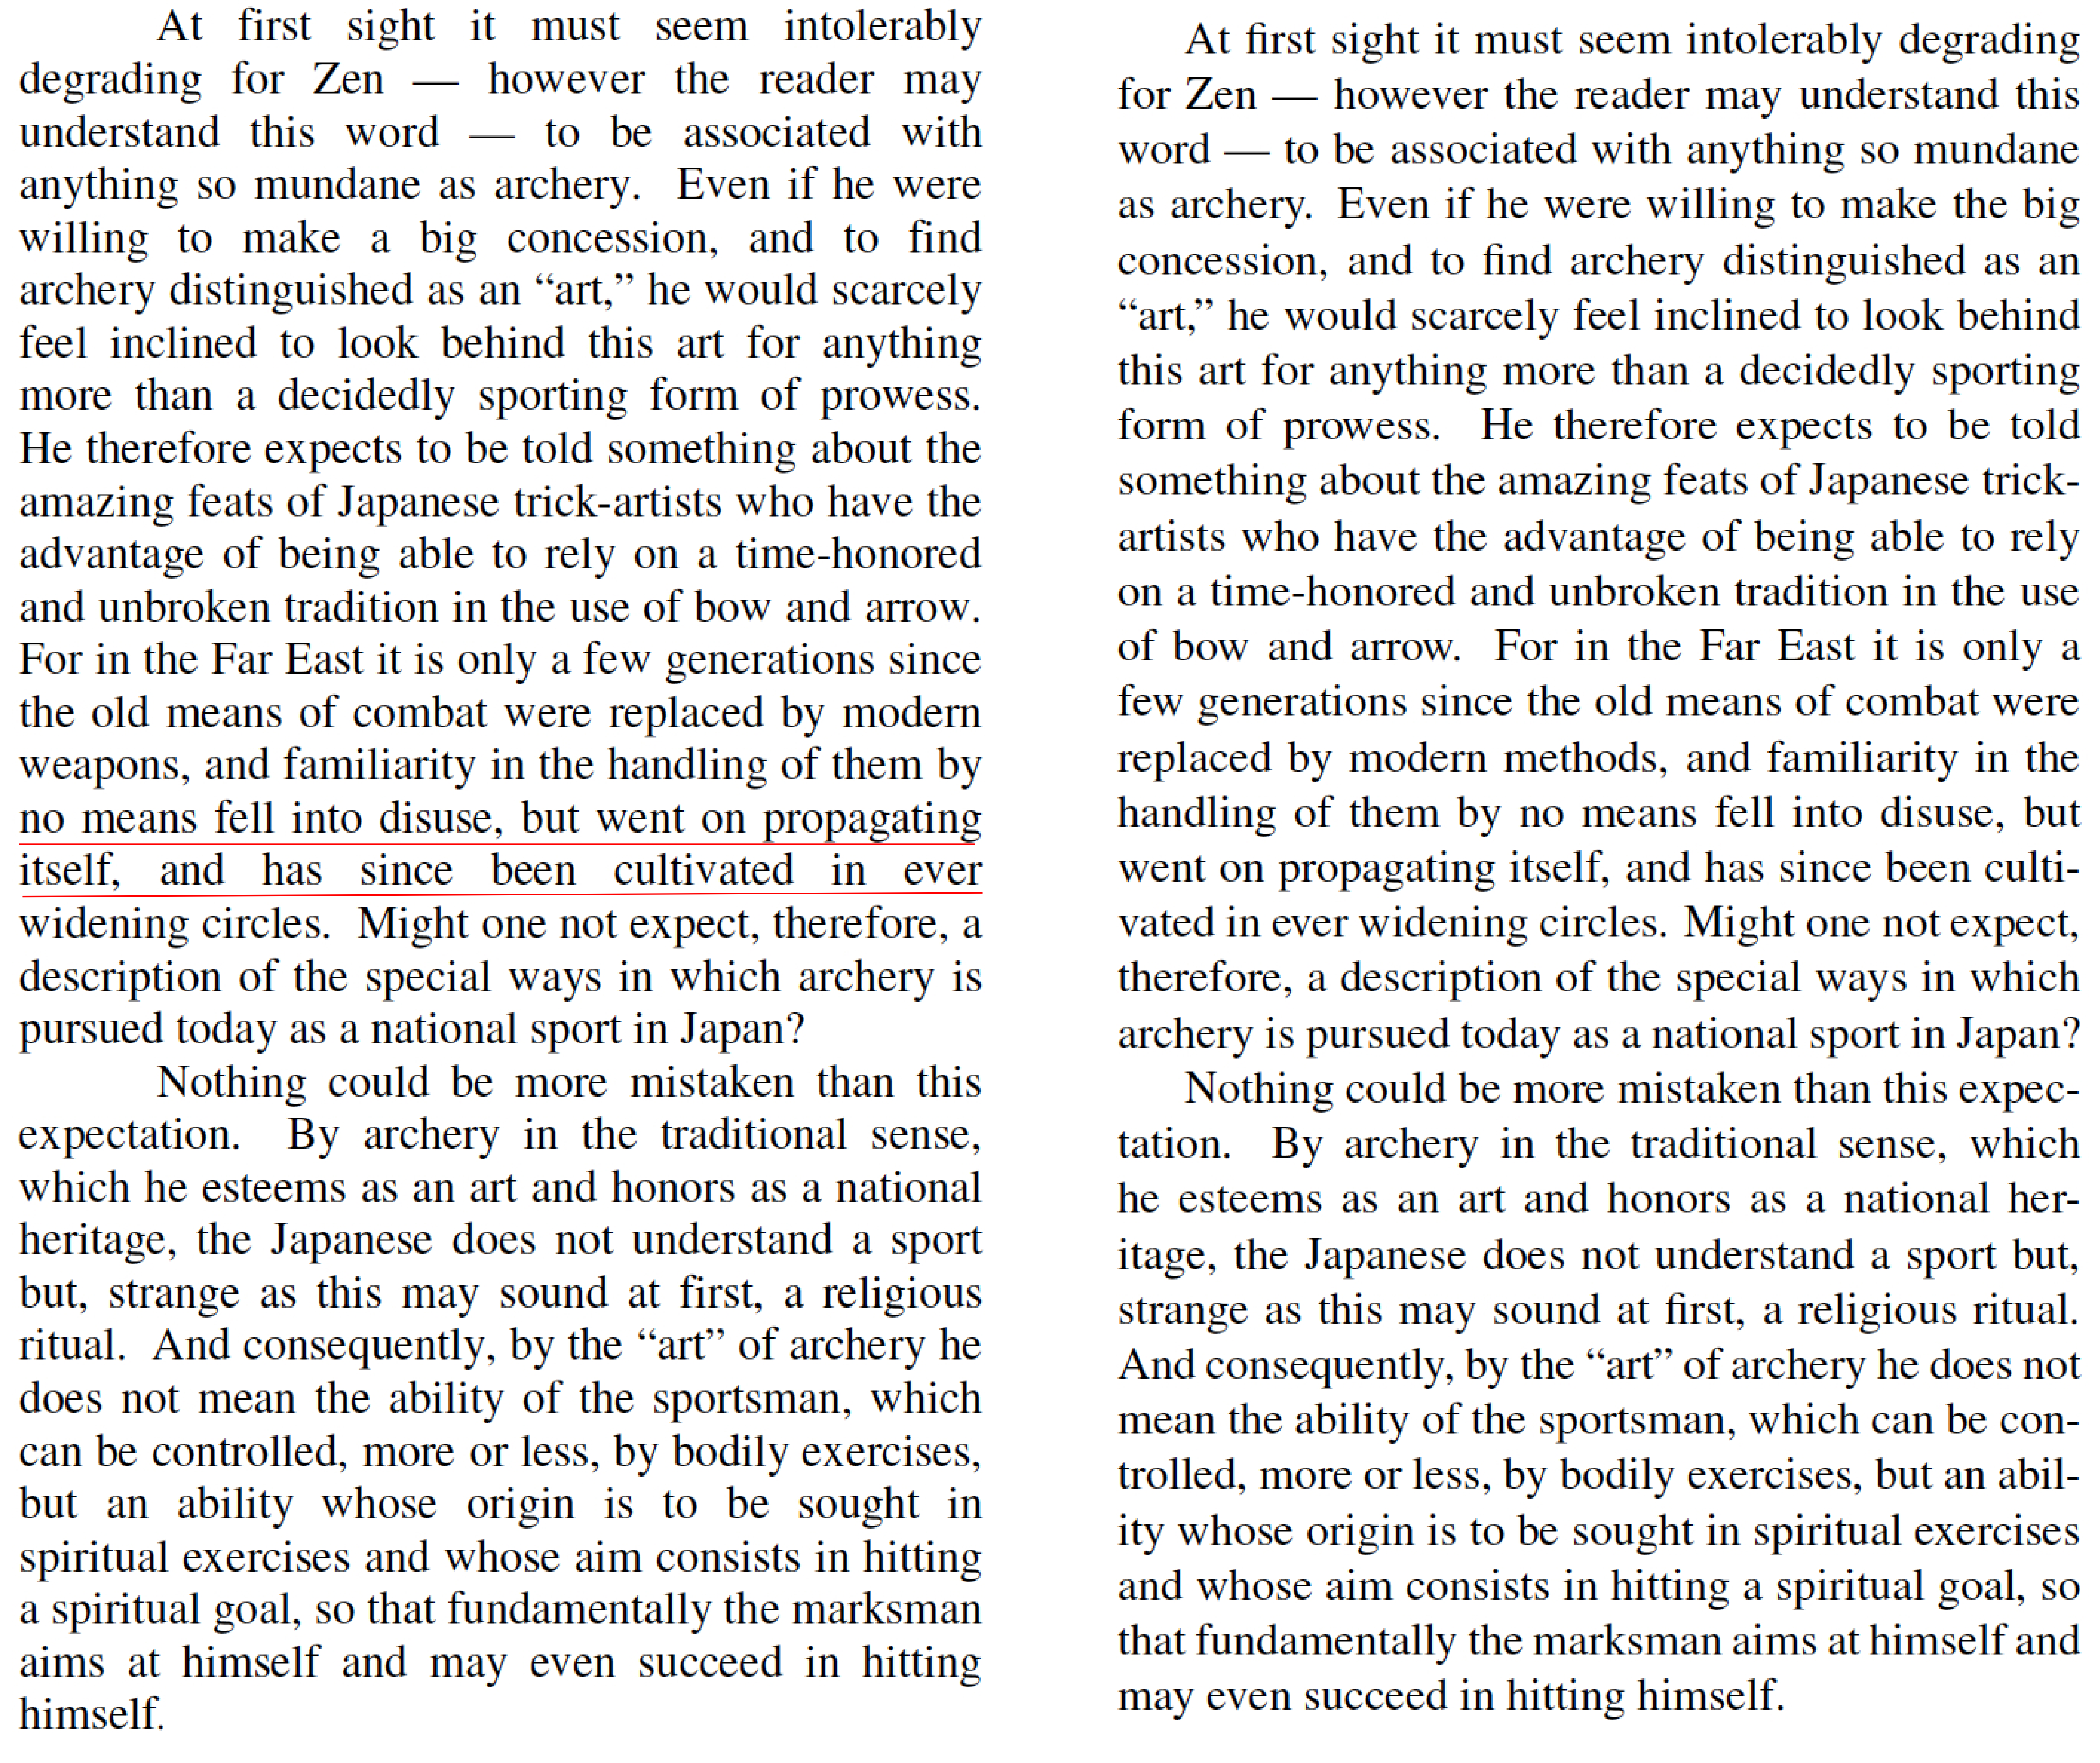
\includegraphics[height=0.85\textheight]{figs/LaTeX_Word.png}
\end{figure}
\end{frame}

%*******************************************************************************
%******************************* Frame *****************************************
%*******************************************************************************
\begin{frame}{Ligatures}
\begin{figure}
\centering

\includegraphics[width=0.7\textwidth]{figs/ligatures_word.png}
\caption{MS Word}
\end{figure}
\begin{figure}
\centering

\includegraphics[width=0.7\textwidth]{figs/ligatures_latex.png}
\caption{\LaTeX}
\end{figure}
\flushright
D.Taraborelli (2008), The Beauty of \LaTeX
\end{frame}

%*******************************************************************************
%******************************* Frame *****************************************
%*******************************************************************************
\begin{frame}
\frametitle{Developers}
\begin{itemize}
\item
\parbox{0.25\textwidth}{
	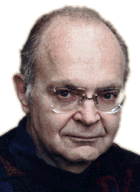
\includegraphics[width=0.15\textwidth]{figs/Donald_Knuth.png}}
\parbox{0.65\textwidth}{Donald Knuth, 1977, \TeX ~Version 3.141592}
\item
\parbox{0.25\textwidth}{
	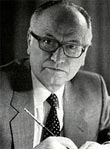
\includegraphics[width=0.15\textwidth]{figs/Hermann.jpg}}
\parbox{0.65\textwidth}{Hermann Zapf}
\item
\parbox{0.25\textwidth}{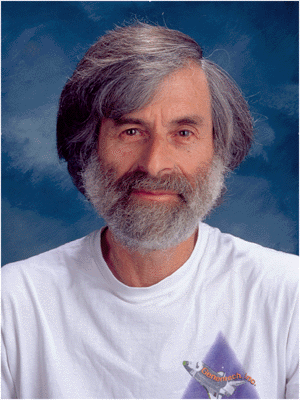
\includegraphics[width=0.15\textwidth]{figs/Leslie.png}}
\parbox{0.65\textwidth}{Leslie Lamport, \LaTeX2e}
\end{itemize}
\end{frame}

%*******************************************************************************
%******************************* Frame *****************************************
%*******************************************************************************
\begin{frame}{How \LaTeX works? - The Magic}
\begin{itemize}
\item You write your document in \texttt{plain text} with \cmd{commands} that
describe its structure and meaning.
\item The \LaTeX program processes your text and commands to produce a
beautifully formatted document.
\end{itemize}

\centering
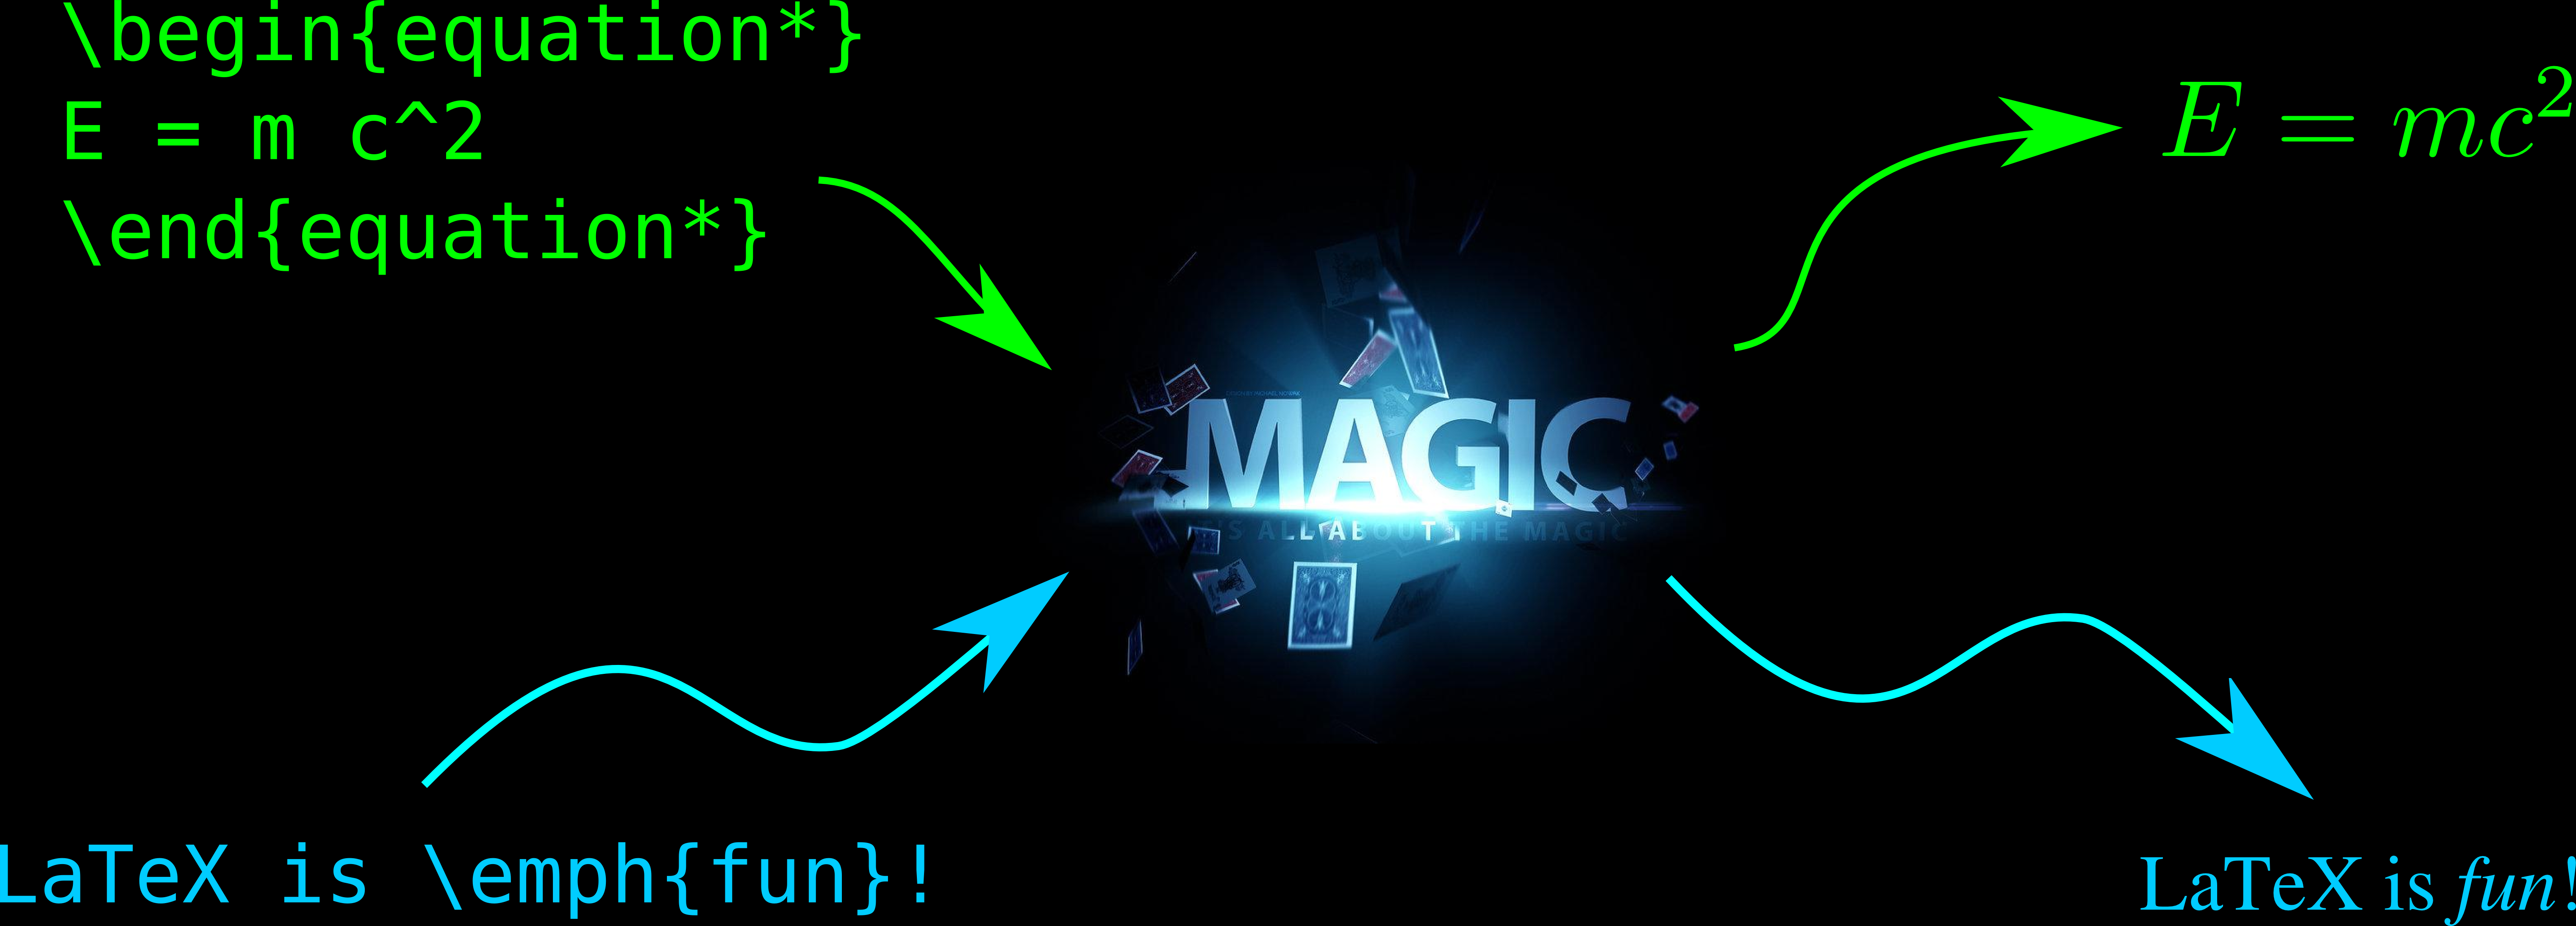
\includegraphics[width=0.95\textwidth]{figs/magic.png}
\end{frame}

%*******************************************************************************
%******************************* Frame *****************************************
%*******************************************************************************

\begin{frame}{\LaTeX Pros and Cons}
\textbf{Pros}
\begin{itemize}
\item    It's free and works on Macs, Windows, Unix/Linux.
\item    LaTeX files are ASCII and are portable.
\item    The typesetting is better, especially the maths.
\item    Style changes are neater in LaTeX. 
\end{itemize}
\textbf{Cons}
\begin{itemize}
\item    Special/Modern Font selection is difficult, but one can use XeTeX.
\item    LaTeX encourages (almost insists on) structured writing and the 
separation of style from content. This is not the way that many people 
(especially non-programmers) are used to working.
\item    Without a WYSIWYG front end, it's not always easy to find out how to 
do things.
\end{itemize}
\end{frame}


%*******************************************************************************
%******************************* Frame *****************************************
%*******************************************************************************
\begin{frame}[fragile]{More examples of commands and their output\ldots}
\begin{exampletwoup}
\begin{itemize}
\item Despicable Me
\item Wall-E
\item Tangled
\end{itemize}
\end{exampletwoup}
\vskip 2ex
\begin{exampletwoup}
\begin{figure}

\includegraphics{figs/minion}
\end{figure}
\end{exampletwoup}
\vskip 2ex
\begin{exampletwoup}
\begin{equation}
\alpha = \beta + 1
\end{equation}
\end{exampletwoup}
\end{frame}

%*******************************************************************************
%******************************* Frame *****************************************
%*******************************************************************************
\begin{frame}[fragile]{Getting Started}
\begin{itemize}
\item A minimal \LaTeX{} document:
\inputminted[frame=single]{latex}{Hello.tex}
\item Commands start with a \emph{backslash} \keys{$\backslash$}
\item Every document starts with a \cmdbs{documentclass} command.
\item The \emph{argument} in curly braces \keys{\{} \keys{\}} 
tells \LaTeX what kind of document we are creating: an \bftt{article}.
\item A percent sign \keys{\%} starts a \emph{comment} --- \LaTeX
will ignore the rest of the line.

\end{itemize}
\end{frame}

%*******************************************************************************
%******************************* Frame *****************************************
%*******************************************************************************
\begin{frame}{Let's try that \dots}
\begin{itemize}
\item write\LaTeX{} is a website for writing documents in \LaTeX.
\item It `compiles' your \LaTeX{} automatically to show you the results.
\vskip 2em
\begin{center}
\fbox{\href{\wlnewdoc{Ex1-Hello/Ex1-hello.tex}}{%
Click here to open the example document in \wllogo{}}}
\\[1ex]\scriptsize{}Or go to this URL: 
\url{\wlserver/docs/1778557gcvcyt/clone}\\
For best results, please use \href{http://www.google.com/chrome}{Google Chrome} 
or a recent \href{http://www.mozilla.org/en-US/firefox/new/}{FireFox}.
\end{center}
\item If you would like to try out the exercise on your machine. Go to 
\cmmd{Exercises / Ex1\_Hello.tex}
\end{itemize}
\end{frame}

%*******************************************************************************
%******************************* Frame *****************************************
%*******************************************************************************
\section{Structure}

%*******************************************************************************
%******************************* Frame *****************************************
%*******************************************************************************
\begin{frame}{LaTeX Structure - The Magic}
\begin{figure}
\centering
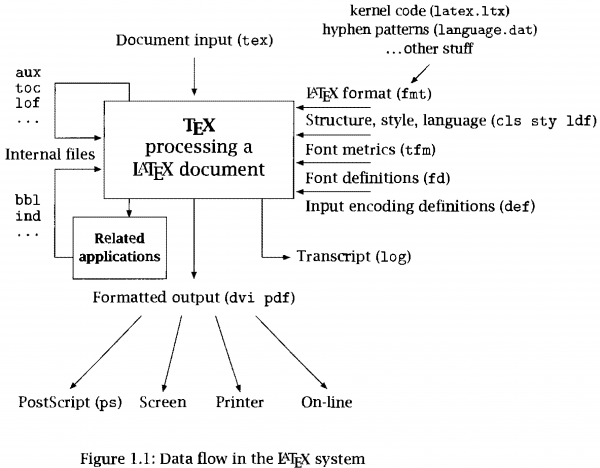
\includegraphics[height=0.95\textheight]{figs/LaTeX.png}
\end{figure}
\end{frame}


%*******************************************************************************
%******************************* Frame *****************************************
%*******************************************************************************
\begin{frame}{$\backslash$documentclass\{\}}

\begin{table}
\renewcommand{\arraystretch}{1.5}
\begin{tabularx}{0.9\textwidth}{l X}
\toprule
minimal & Is as small as it can get. For debugging purposes.\\ 
letter & For writing letters. \\ 
article & articles in journals, documentation, invitations, \dots \\ 
proc & A class for proceedings based on the article class.\\ 
report & For longer reports containing several chapters \dots \\
book & For real books.\\
memoir & For advanced book style. \\
beamer& For writing presentations \\ \bottomrule
\end{tabularx}
\end{table}
\end{frame}


%*******************************************************************************
%******************************* Frame *****************************************
%*******************************************************************************
\begin{frame}[fragile]{Typesetting Caveats}
\small
\begin{itemize}
\item Quotation marks are a bit tricky: use a backtick \keys{\`{}} on the 
left and an apostrophe \keys{\'{}} on the right.

\begin{exampletwouptiny}
Single quotes: `text'.

Double quotes: ``text''.
\end{exampletwouptiny}

\item Some common characters have special meanings in \LaTeX:\\[1ex]
\begin{tabular}{cl}
\keys{\%} & percent sign (comment)             \\
\keys{\#} & hash sign (macro parameter \#1)    \\
\keys{\&} & ampersand (align)                  \\
\keys{\$} & dollar sign (in-line math)         \\
\end{tabular}
\item If you just type these, you'll get an error. If you want one to appear in
the output, you have to \emph{escape} it by preceding it with a backslash.

\begin{exampletwoup}
\$\%\&\#
\end{exampletwoup}
\end{itemize}
\end{frame}

%*******************************************************************************
%******************************* Frame *****************************************
%*******************************************************************************

\begin{frame}{Exercise 2: Typesetting}

\begin{block}{Typeset this in \LaTeX:
\footnote{\url{http://en.wikipedia.org/wiki/Economy_of_the_United_States}}}
In March 2006, Congress raised that ceiling an additional \$0.79 trillion to
\$8.97 trillion, which is approximately 68\% of GDP. As of October 4, 2008, the
``Emergency Economic Stabilization Act of 2008'' raised the current debt ceiling
to \$11.3 trillion.
\end{block}
\vskip 2ex
\begin{center}
\fbox{\href{\wlnewdoc{Ex2-Typeset/Ex2-Typeset.tex}}{%
Click to open this exercise in \wllogo{}}}
\end{center}

\begin{itemize}
\item Hint: watch out for characters with special meanings!
\item Once you've tried,
\fbox{\href{\wlnewdoc{Ex2-Typeset-solution/Ex2-Typeset-solution.tex}}{%
click here to see my solution}}.
\end{itemize}
\end{frame}


%**********************************************FRAME***************************************
\begin{frame}{Acknowlegements}
This \LaTeX for Beginners course is loosely based on and examples from:
\begin{itemize}
\item John Miller's An interactive introduction to \LaTeX: 
\href{https://www.writelatex.com/blog/7}{https://www.writelatex.com/blog/7}
\item WikiBook on \LaTeX: 
\href{https://en.wikibooks.org/wiki/LaTeX}{https://en.wikibooks.org/wiki/LaTeX}
\item Share\LaTeX Learn: 
\href{https://www.sharelatex.com/learn}{https://www.sharelatex.com/learn}
\item CUED Textprocessing: \href{http://www.eng.cam.ac.uk/help/tpl/textprocessing/}{http://www.eng.cam.ac.uk/help/tpl/textprocessing/}
\item UCS Course on \LaTeXe: \href{http://www.ucs.cam.ac.uk/docs/course-notes/unix-courses/earlier/latex}{http://www.ucs.cam.ac.uk/docs/course-notes/unix-courses/earlier/latex}
\end{itemize}
\end{frame}

\end{document}
